\section{Theorie}
\label{sec:Theorie}

\subsection{Einleitung}
\label{subsec:Einleitung}
Myonen zählen als Elementarteilchen, die nicht der Starken Wechselwirkung unterliegen, zur Gruppe der Leptonen.
Sie tragen eine Ladung und wechselwirken daher auch mit elektromagnetischen Feldern.
Im Vergleich zum Elektron besitzt das Myon eine ca. 207 mal größere Ruhemassen und ist nicht stabil.
Der Zerfall von Myonen folgt dem Schema
\begin{align}
\mu^- \longrightarrow e^- + \bar{\nu_e} + \nu_\mu
\end{align}
bzw.
\begin{align}
\mu^+ \longrightarrow e^+ + \nu_e + \bar{\nu}_\mu
\end{align}
im Fall des Antimyons.
Mit dem im Folgenden untersuchten Versuch soll die Lebensdauer von Myonen bestimmt werden.
Diese ist durch den Erwartungswert der Lebensdauerverteilung einzelner Myonen gegeben.
\subsection{Lebensdauer instabiler Teilchen}
\label{subsec:Lebensdauer instabiler Teilchen}
Da Teilchenzerfälle rein statistische Prozesse sind, wird für die Zerfallswahrscheinlichkeit $dW$ eines Teilchens im Zeitraum $dt$ der Ansatz
\begin{align}
\text{d} W = -  \lambda \text{d} t
\end{align} 
gemacht.
Insbesondere hängt die Zerfallswahrscheinlichkeit nicht von der Anzahl der vorhandenen Teilchen $N$ ab.
Für die Änderung der Teilchenzahl im Zeitraum $dt$ gilt also
\begin{align}
\text{d} N = - N \text{d} W = - N \lambda \text{d} t\text{ ,}
\end{align} 
was durch Integration auf 
\begin{align}
N(t)=N_0\exp(-\lambda t)
\end{align}
führt.
Um auf die Verteilungsfunktion zu schließen, muss betrachtet werden wie viele Teilchen eine Lebensdauer im Bereich von $t$ bis $dt$ haben.
Diese Betrachtung führt auf eine Exponentialverteilung
\begin{align}
\text{d} N(t)=N_0 \lambda \exp(-\lambda t) \text{d} t \text{ .}
\end{align}
Die Lebensdauer $\tau$ eines Teilchens ist der Erwartungswert dieser Verteilung, welcher gerade $\tau = \frac{1}{\lambda}$ ist.
\cite{sample}
\subsection{Messung der Lebensdauer}
\label{subsec:Messung der Lebensdauer}
Der Nachweis von in der Erdatmosphäre erzeugten Myonen soll mit einem organischen Szintillations Detektor geschehen, da organische Szintillatoren eine besonders kurze Ansprechzeit von wenigen Nanosekunden besitzen.
Ein in den Detektor einfallendes Myon gibt seine kinetische Energie an einzelne Atome des Detektors ab.
Die dadurch angeregten Moleküle gehen unter Emission von Photonen in ihre Grundzustände über.
Auf diese Weise entsteht ein Photonenschauer, der von einem Sekundärelektronenvervielfacher (SEV) nachgewiesen wird.
Gibt ein Myon seine gesamte kinetische Energie an die Moleküle des Detektors ab, so zerfällt es innerhalb des Detektors.
Beim Zerfall des Myons in ein Elektron und ein Neutrino wird die Ruhemasse des Myons teilweise in kinetische Energie des Elektron überführt.
Dieses ist daher in der Lage wiederum Atome des Detektormaterials anzuregen, was wie oben beschrieben zu einem weiteren Photonenschauer führt.
Der zeitliche Abstand zwischen zwei solchen Signalen entspricht dann der Lebensdauer eines bestimmten Myons.
Der SEV besitzt den Nachteil, dass thermische Effekte häufig zur Emission von Elektronen führen.
Durch den Einsatz von zwei SEV und einer Koinzidenzschaltung wird verhindert, dass auf diese Weise entstehende Signale an die im Folgenden beschriebene Schaltung zur Messung der Lebensdauer weitergeleitet werden.
Die Koinzidenzschaltung gibt ein Signal nur dann weiter, wenn dieses von beiden SEV nahezu gleichzeitig gesendet wird.
Da sich die spontane Emission von Elektronen beider SEV nicht gegenseitig bedingt, kann so ein Großteil der Störeffekte gefiltert werden.
Um einheitliche Signale zu gewährleisten wird zwischen die SEV und die Koinzidenzschaltung jeweils ein Diskriminator mit variabler Schwelle geschaltet.
Dieser wandelt die Signale der SEV in Rechtecksignale nach dem NIM-Standard um und ermöglicht der Koinzidenzschaltung daher die Signale der beiden SEV bestmöglich zu vergleichen.
Zusätzlich werden die Signale der SEV durch die Schwelle des Diskriminators bereits vorgefiltert.
Die beiden Schwellen sollten so eingestellt werden, dass beide Diskriminatoren die gleiche Anzahl von Signalen an die Koinzidenzschaltung weiterleiten.

Da die Lebensdauer von Myonen im Vergleich zur Häufigkeit des Eintretens von Myonen in den Detektor klein ist, kann der zeitliche Abstand nach der Stoppuhr-Methode gemessen werden.
Das bedeutet, dass eine Uhr mit jedem registrierten Signal abwechselnd gestartet bzw. gestoppt wird.
Bei Verwendung dieser Methode treten jedoch zwei wesentliche Probleme auf.
In dem Fall, dass ein Myon nicht im Detektor zerfällt würde kein zweites Signal von diesem Myon ausgehen, welches die Zeitmessung beendet.
Für die Versuchsapparatur wirkt es in diesem Fall so, als würde das Signal, welches das nächste Myon bei seinem Eintritt in den Detektor erzeugt, vom Zerfall des vorherigen Myons stammen.
Da das zu groben Verfälschungen der Messergebnisse führen würde, wird die Suchzeit $T_s$ eingeführt.
Diese bestimmt wie lange die Uhr auf ein Stoppsignal wartet.
Ist die Suchzeit vorüber führt das nächste Signal zum erneuten Starten der Uhr.
Das zweite Problem ist, dass zwei Myonen in einem zeitlichen Abstand in der Größenordnung der zu messenden Lebensdauern in den Detektor eintreten.
Dieses Problem bleibt nach Einführung der Suchzeit bestehen.
Das Eintreten von Myonen in den Detektor ist jedoch statistisch so verteilt, dass der durch dieses Problem erzeugte Fehler alle gemessenen Zeiten auf die gleiche Weise betrifft.
Nach Berechnung dieses gleichmäßig verteilten Fehlers, kann der Fehler von den Zählergebnissen der verschiedenen Lebensdauern abgezogen werden.
Eine mögliche Versuchsanordnung zur Messung der Lebensdauer nach der Stoppuhr-Methode greift auf die Kombination aus einem Zeit-Amplituden-Konverter (TAC) und einem Vielkanalanalysator (VKA) zurück.
Die im Folgenden beschriebene und in Abbildung \ref{fig:t:1} dargestellte Schaltung leitet Start- und Stoppsignale an den TAC weiter, welcher ein zur Zeit zwischen einem Start und einem Stopp Signal proportionales Spannungssignal an den Vielkanalanalysator weiter gibt.
\begin{wrapfigure}{r}{0.5\textwidth}
\centering
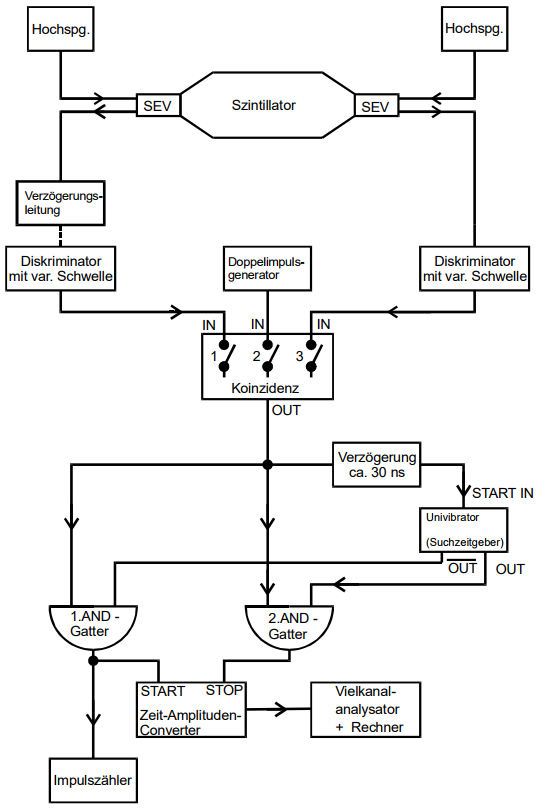
\includegraphics[width=0.5\textwidth]{content/skizzen/aufbau.png}
\caption{Schaltbild der Apparatur zur Messung der Lebensdauer von Myonen \cite{sample}. Die Leitung zwischen dem 2. AND-Gatter und dem Impulszähler stammt nicht aus dem Original, sondern wurde nachträglich eingefügt.}
\label{fig:t:1}
\end{wrapfigure}
Dieser ordnet jedem Signal entsprechend seiner Größe einen Kanal innerhalb eines Datensatzes zu und erhöht den Wert des entsprechenden Kanals um Eins.
Die Anzahl der Signale, die in einem bestimmten Kanal gespeichert werden, entspricht also der Häufigkeit des Auftretens eines Signals mit dieser Lebensdauer.
Um die Suchzeit in die Schaltung zu implementieren wird eine Monostabile Kippstufe verwendet.
Diese besitzt einen Eingang und zwei Ausgänge.
Liegt am Eingang keine Spannung an steht ein Ausgang auf H und einer auf L.
Sobald ein Spannungssignal den Eingang erreicht werden beide Ausgänge für die einstellbare Suchzeit auf den jeweils anderen Wert umgeschaltet.
Ein von der Koinzidenzschaltung abgegebenes Signal wird an zwei verschiedene AND-Gatter und mit einer Verzögerung von $\SI{30}{\nano\second}$ an die Monostabile Kippstufe weiter gegeben.
Der ohne anliegende Spannung am Eingang auf H stehende Ausgang ist mit dem ersten AND-Gatter verbunden, sodass dieses das Signal an den Starteingang des TAC und einen Impulszähler weiterleiten kann.
Während der Suchzeit steht nun der andere Ausgang der Monostabilen Kippstufe auf H, sodass ein während der Suchzeit von der Koinzidenzschaltung abgegebenes Signal durch das zweite AND-Gatter, aber nicht durch das erste, zum Stoppeingang des TAC geleitet wird.
Gibt die Koinzidenzschaltung während der Suchzeit kein Signal ab, so gelangt das nächste Signal wieder zum Starteingang des TAC.

\cite{sample}
